\section{\espina{} views}

\espina{} has two different types of view to represent the loaded images: a planar, 
two-dimensional view and a three-dimensional view. By default the program shows three
planar views (which correspond to the axial, coronal and sagittal views) and one
three-dimensional view. \\
Although both are interactive all work (segmentation, editing and analysis) is
performed in the planar view, leaving the three-dimensional view solely for
a three-dimensional representation of the results. \\
Both type of views can be docked into the main \espina{} window or can become floating
widgets if the user click and drags in the view title to it's new position. And can become
docked widgets if the user drags it back to the \espina{} main window. \\

\subsection{Two-dimensional view}

The two-dimensional views are formed by a view area and a slider bar. The view area is
used to operate with the channel or segmentations, and the slider is used to move through
the stack of images in the direction of the view. Alternatively you can use the mouse wheel
to get the same result as using the slider.\\

\begin{figure}[H]
\centering
\includegraphics[scale=0.33]{fig/2DView}
\caption{Two-dimensional view, with thumbnail and ruler.}
\end{figure}

When there is no tool or widget in use the user can select a segmentation by left clicking
on it, or select a group of segmentations if the shift key is holded down while left clicking.\\
To move over the plane the user must click and hold the middle button of the mouse and move
the mouse in the direction he wants to translate the plane. To zoom the image, the operation is
similar to he previous one, but with the right button of the mouse. \\
Over the view area there can be two additional items: the size ruler, that gives us a measure of
size and distance, and the slice thumbnail, that appears when the image is too big to completely
fit into the view area and shows us the part of the slice we are looking at. Movement over the
plane is also possible left clicking on the thumbnail when it's present.

\subsection{Three-dimensional view}

The three-dimensional view is formed by a view area and a set of buttons on the right and 
left of the bottom of the view. \\
As noted before, the three dimensional view shows a interactive representation of the
segmentations and other data like, for example, the crosshair position.\\
The operation of the three-dimensional view is similar to what was explained in the previous
subsection for the planar view. Translating and zooming works the same way (with the exception
that now the mouse wheel can be also used to zoom the scene), and to rotate the representation
the user must hold down the left mouse button and move it in the direction he wants to rotate.\\

\begin{figure}[H]
\centering
\includegraphics{fig/VolumeView}
\caption{Three-dimensional view widget.}
\end{figure}

The buttons at the bottom-left of the view allows the user to export the representations as a image
or a three-dimensional scene.\\
\vspace{0.2cm}

\begin{tabular}{| m{1.3cm} | m{12cm} |}
\hline
\textbf{Button} & \textbf{Description}\\
\hline
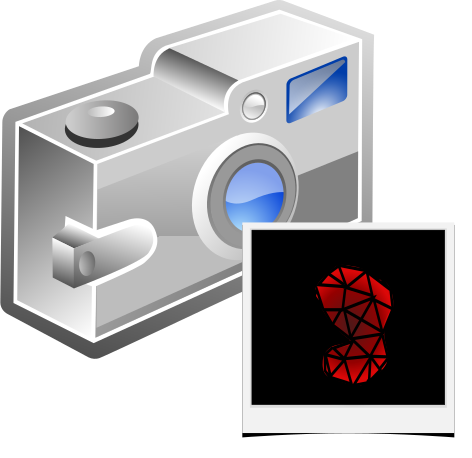
\includegraphics[width=0.7cm]{../../frontend/rsc/snapshot_scene} & 
\textbf{Take Snapshot}: Save an snapshot of the current view. Supported formats:
\begin{itemize}
\item JPG (Joint Photographic Experts Group)
\item PNG (Portable Network Graphics)
\end{itemize}\\
\hline
\includegraphics[width=0.7cm]{../../frontend/rsc/export_scene} &
\textbf{Export 3D Scene}: Export current displayed scene into a 3D compatible format. Supported formats:
\begin{itemize}
\item POV (Persistence Of Vison)
\item VRML (Virtual Reality Modelling Languange)
\item X3D (XML-based format, the successor of VRML)
\end{itemize}
\begin{bclogo}[couleur = yellow!33, logo=\bcattention]
{Note} Only the mesh objects of the scene are exported, volumetric objects are not. This is a limitation of the destination formats.
\end{bclogo}\\
\hline
\end{tabular}
\vspace{0.3cm} 

On the bottom-right there is the set of buttons called ``renderers''. A renderer is
a way to represent information that can be toggled (activated or deactivated). By
default \espina{} shows three renderers.

\begin{tabular}{| m{1.3cm} | m{12cm} |}
\hline
\textbf{Button} & \textbf{Description}\\
\hline
\includegraphics[width=0.7cm]{../../frontend/rsc/show_planes} &
\textbf{Crosshair Renderer}: Toggle channel's crosshair planes visibility.\\
\hline
\includegraphics[width=0.7cm]{../../frontend/rsc/mesh} &
\textbf{Mesh Renderer}: Toggle segmentation's mesh rendering.\\
\hline
\includegraphics[width=0.7cm]{../../frontend/rsc/voxel} &
\textbf{Volumetric Renderer}: Toggle segmentation's volumetric rendering.\\
\hline
\end{tabular}
\vspace{0.3cm} 

Additionally plugins can add buttons to this set of renderers. Refer to the plugin
documentation for a description of those.

